\chapter{Evaluation}
\renewcommand{\baselinestretch}{\mystretch}
\label{chap:evaluation}
\section{Overview}
This evaluation section will look at the results of the tests designed in the previous section, producing metrics of exactly how fast and scalable this implementation is. Comparisons will be drawn against the benchmark system noting any differences in resource profile and speed. In the later section the algorithm will be considered in terms of real genomes and the size of this problem set as well as comparing the processor with other algorithms that were introduced in the related work section.
%\setlength{\parindent}{0pt}
\section{Comparison to Benchmark Algorithm}
\subsection{Resource Usage}
The memory utilisation tested in the performance characteristics section showed that memory usage scaled up proportional to the read length for the algorithm. This is expected due to the design of full read length sized FIFO memory storage. It can be noted however, that even read lengths of 1,600 gave only 37,360 memory bits, less than 20\% of the memory available on the DE0 FPGA. This scale of read length is significantly above the maximum lengths achieved with current pyrosequencing techniques, the maximum of which are only 1,000. As a result it's perfectly safe to allow full sequence buffering, which removes any risks from having a slower throughput in the comparison engine that the input source. 

In terms of logic utilisation, figures \ref{fig:fpgacount}, \ref{fig:pix}, \ref{fig:read}, \ref{fig:lib} show that the implementation uses around 4 thousand logic elements for the control and interface logic on each FPGA. This equates to around 2 pixels on an average device. As a result, the increase in processing power when moving from one device to two effectively $2\times \text{pixel count} - 4 $, and this overhead does not increase on a per device basis when adding more devices above this. This means that moving from a four device cluster to a five device cluster does not increase the logic on the original four devices at all, although memory usage increases marginally on the master. This makes the design particularly scalable in terms of resources.

When looking at how logic usage scales with pixel count, it can be seen from figure \ref{fig:pix} that the relationship is linear. Each pixel adds around 1,500 logic elements to the design and this relationship does not change depending on how many devices are used. This is the type of scaling that was expected and is ideal for maximising parallelism. It is important to note however that increased pixels does not necessarily directly relate to increased processing power as algorithm speed may be impacted.


Whilst it's theoretically possible to scale up the number of devices quite significantly, moving to dozens of devices before the clock skew issues would lower the clock frequency, this is still not the scale of the massively parallel operation the detection devices work on. Instead, larger devices such as the Terasic CYCLONE V GX development kit, would be able to massively scale up the computational power. As well as dedicated clock ports, the High Speed Mezzanine Connectors (HSMC) give the opportunity to increase the inter-FPGA communications which was cited as a key limitation in the hardware design section. Each of these devices is capable of fitting in the order of 100 pixels based on the tests shown earlier. As such, a large cluster of these devices would be capable of comparing thousands of pixels of data in parallel. It is important to note however, this is still not of the order of the very highest density chips. 

The scalability of the algorithm in terms of how many sequences can be shared between pixels and therefore how many parallel calculations can be done is a severe limitation. The number of inter-FPGA communication pins are always a hard limit, and with 30 pins required for the data IO communication, the number of pins required for the ring network can often be a limiting factor. This is therefore likely to be a key motivating factor when choosing hardware on which this algorithm can be implemented. There are solutions to this problem however, like the HSMC ports mentioned earlier. This does not prevent more pixels to be used on a single device however, and for this reason, the approach of smaller pixels with more comparison cycles may be necessary. The inter-pixel communication can be lowered by reducing the comparisons in parallel, this pays off both in number of inter-device connections as well as simplifying the logic of each pixel and therefore fitting more pixels per device. This does negatively impact the number of comparison cycles that need to be done however, and a balance must be made. This would normally be done by identifying the number of pixels absolutely necessary and the absolute maximum inter-device ports available. 


\subsection{Speed}


On smaller FPGAs such as the DE0 that was used for testing, only around 9 pixels can be fitted on a single device. This meant the 3 device cluster was capable of running a 27 pixel array, with speed of comparison as short as 31ms for the full comparison. This is equivalent to 478,000 comparisons per second making this array very powerful. The advantage of this system is the massive parallelism, an all against all comparison has a computational complexity of $O(n^2)$. For large n this becomes very slow, however for large n, a larger device can be used and the computation time scales with $O(\frac{n^2}{m})$ where m is the number of pixels. This significantly speeds up the operation. 


Another important element of speed is the effectiveness of adding an FPGA delay, as discussed earlier, a each extra FPGA device slows the cycle count by 2 cycles. Ignoring the effect of clock frequency, as long as the number of pixels per FPGA is greater than 2, an extra device will always increase processing power. However, clock frequency cannot be ignored, as all devices must work from the same clock, and whilst the path from one FGPA to another may not increase, attempting to keep the path of the clock the same to all devices would be extremely difficult. This means there would be clock skew between devices which limits how fast the clock frequency may be. As a result of this the best method for this algorithm is small clusters of high-powered devices. 


As discussed in the motivation section, the detection chip is using chemical processes to sequence the DNA which is significantly slower than the processing speed of a CMOS chip. The detection time period of around 4~s is orders of magnitude slower than the comparison engine, with can operate with a clock period of as little as 32~ns. The time to do a single comparison cycle has been shown to take $N + 2T $ where N is the overlap count and T is the number of FPGAs in the array. These measurements show that the comparison engine is more than capable of operating at speeds much faster than the detection chips. This is not enough however, for real-time processing. An important element of the comparison engine is the number of parallel comparison engine pixels that can be used within the circuit. The scale of the comparison engines pixels is no where near enough to allow true real-time stream processing of the detection chip data. In order to achieve this directly, modifications would have to be made to the algorithm as covered in the future work section.

\section{Comparison to Existing Technology}

In the testing section of the report figure \ref{table:speed} the speed of the algorithm was shown for varying read lengths with 27 pixels. At a read length of 50 the comparison engine processed ($27^2$) comparisons in 31~ms or $42~{\mu}s$ per comparison. It is possible to compare this to the assembly speeds of the algorithms discussed in the related work section. 

In the paper comparing sequence assemblers it was found the quality of recombined sequences generally did not improve about 40x coverage depth, meaning that the short reads defined the full sequence 40 times \cite{lin2011comparative}. For genome lengths of 4.6~million in the case of E.Coli, this would mean $\frac{4.6\times 10^6 \times 40}{50} = 3.68~\text{million}$ reads with read length 50. When taking into account these facts, the total estimated time for the DE0 FPGA cluster to do this comparison would be $(3.68\times 10^{6})^2 \times 42 \times 10^{-6} = 5.6\times10^{9}~\text{s}$. This can be compared to the times listed in figure \ref{fig:comp}, for the other comparison engines. unfortunately this indicates that fast sequencing for full genomes is unrealistic on a 3 DE0 based cluster. This however, is unsurprising as this cluster is extremely low cost when compared to the hardware set up for testing. The testing of the other solutions was conducted on a cluster of 8 computers each of which had 2 quad-core 2.4~GHz processors. This meant that each of these solutions was using 64 processors in parallel to achieve these results. As a result it is unrealistic for this hardware to compare to those benchmarks. When considering a true comparison with this massive assembly problem a more powerful cluster would need to be built.



A cluster of only 3 DE0 boards would more realistically work in real-time for much smaller data sets, in the order to 10kbp, where complete comparison for a 40 times coverage 50 read length would only take 1.68~s. The cluster built in this project was an extremely small implementation of the cluster design, and is unsurprisingly less powerful than the system that was used to test the other algorithms. In order to look at the how a larger cluster would manage larger problem sets, the scalability of the hardware must be analysed.


\subsection{Scalability of hardware}

Predominantly, the limits on the cluster are related to the number of devices used. As discussed earlier, each additional device in the cluster adds a 2 cycle delay per comparison, when scaled across large numbers of devices this forms a limiting constraint on the speed of comparisons. Assuming perfect scaling of the algorithm in terms of frequency, data availability of clock speed the algorithm still tends to a speed limit, this is shown in figure \ref{fig:scale}.

\begin{figure}[!h]
  \centering
  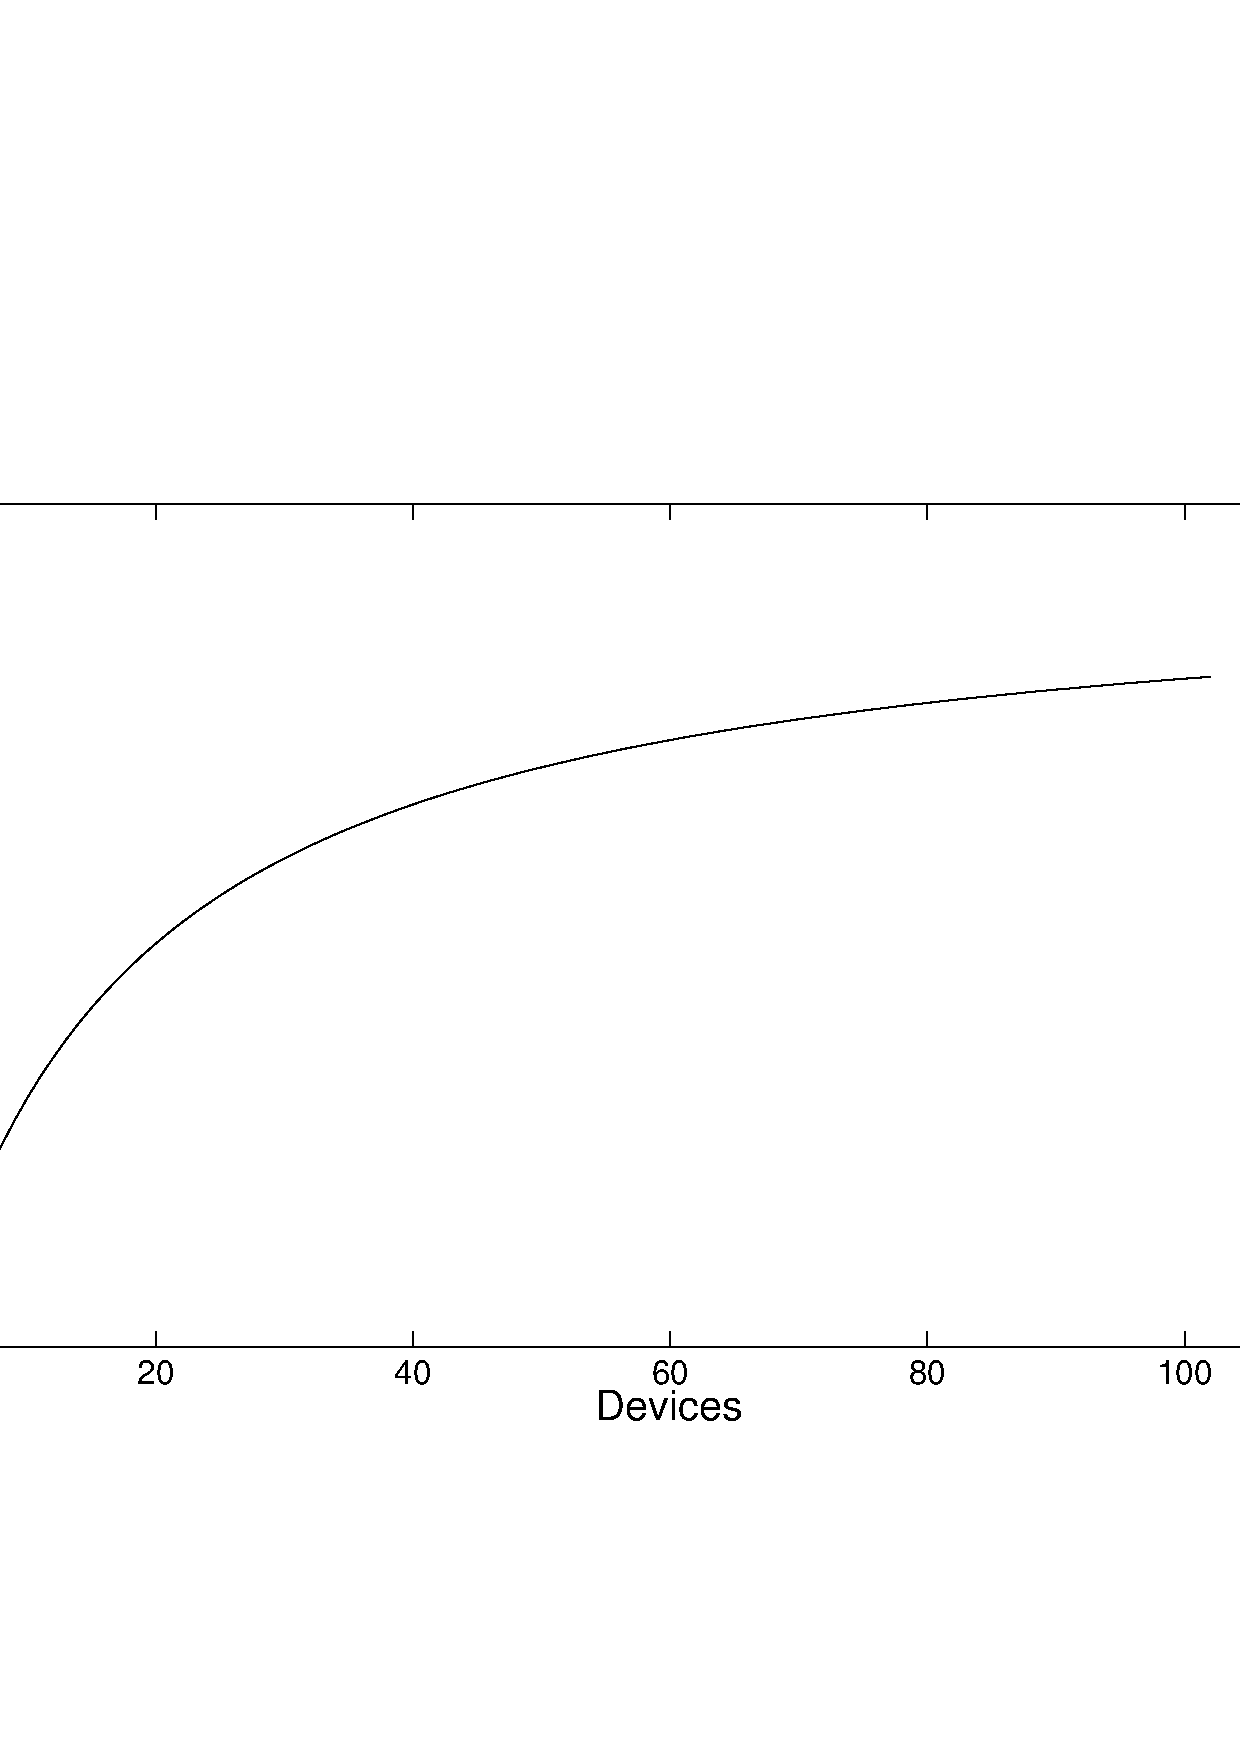
\includegraphics[width=0.7\textwidth]{./figs/scalability.pdf}
  \caption{Scaling of Algorithm with Cluster Size}
    \label{fig:scale}
\end{figure}

This is a hard limit on the scalability of the algorithm due to the delay introduced by the inter-device communication. This only occurs for a very large size of cluster and other factors are likely to come into effect before this. This pattern is  an important factor in scaling the algorithm, as earlier the linear scaling of pixels was discussed in terms of logic utilisation. As logic usage increases, the pixels must be spread across multiple devices, as can be seen in figure \ref{fig:scale} this tends to a limit as the cluster size increases. This means that whilst increasing pixel count per device linearly increases processing power, increasing number of devices tends to a limiting factor due to the length of the comparison cycle increasing. 


The main factor limiting the scalability of this hardware is the clock skew across devices. A shared clock design is naturally limited to how many devices can share the clock synchronously. This largely depends on device hardware, as a clock source coming in to a board via a normal GPIO port is not a high quality clock source, as such it is likely to be skewed and difficult to synchronise across devices. In contrast, higher quality devices have custom clock inputs using Subminiature A connectors designed specifically for the purpose of high quality external clocks. 


An important factor in the scalability of this solution is how efficiently the design can be used to tackle larger problem sizes. This introduces a problem with the comparison engine, it is of comparable speed to the other algorithms presented, especially when considering the disparity in hardware resources. However, scaling the number of comparisons done on the current device is not as simple as doing multiple comparison cycles at full speed. The comparison engine is designed to do a comparison shown in the matrix below, where n is the number of pixels on the cluster.
\begin{center}
$\text{Comparison Matrix} =  \begin{pmatrix}
  F(a_{1},a_{1}) & F(a_{1},a_{2}) & F(a_{1},a_{3}) & \cdots & F(a_{1},a_{n}) \\
  F(a_{2},a_{1}) & F(a_{2},a_{2}) & F(a_{2},a_{3}) & \cdots & F(a_{2},a_{n}) \\
  F(a_{3},a_{1}) & F(a_{3},a_{2}) & F(a_{3},a_{3}) & \cdots & F(a_{3},a_{n}) \\
  \vdots  & \vdots  & \vdots & \ddots & \vdots   \\
  F(a_{n},a_{1}) & F(a_{n},a_{2}) & F(a_{n},a_{3}) & \cdots & F(a_{n},a_{n})
 \end{pmatrix}
$
\end{center}

It is important to notice however, that with the current algorithm it is impossible to only do some of these comparisons, they must all be done in lock-step. As a result performing a comparison of a larger number of sequences is difficult, as a  larger square comparison matrix cannot be formed of repeated smaller square matrices without significant repetition of the same work. This makes using the parallel comparison engine poorly suited to processing larger problemes. In the next section we discuss a method that could be adopted to solve this problem. 